\documentclass[
11pt, % The default document font size, options: 10pt, 11pt, 12pt
codirector, % Uncomment to add a codirector to the title page
]{charter} 
\usepackage{float}

% El títulos de la memoria, se usa en la carátula y se puede usar el cualquier lugar del documento con el comando \ttitle
\titulo{Predicción de histograma dosis-volumen en radioterapia de próstata mediante redes neuronales convolucionales} 

% Nombre del posgrado, se usa en la carátula y se puede usar el cualquier lugar del documento con el comando \degreename
%\posgrado{Carrera de Especialización en Sistemas Embebidos} 
%\posgrado{Carrera de Especialización en Internet de las Cosas} 
\posgrado{Carrera de Especialización en Inteligencia Artificial}
%\posgrado{Maestría en Sistemas Embebidos} 
%\posgrado{Maestría en Internet de las cosas}

% Tu nombre, se puede usar el cualquier lugar del documento con el comando \authorname
% IMPORTANTE: no omitir titulaciones ni tildación en los nombres, también se recomienda escribir los nombres completos (tal cual los tienen en su documento)
\autor{Ing. Natalia Mercedes Espector}

% El nombre del director y co-director, se puede usar el cualquier lugar del documento con el comando \supname y \cosupname y \pertesupname y \pertecosupname
\director{Dr. Flavio Colavecchia}
\pertenenciaDirector{Fundación INTECNUS / CNEA} 
\codirector{Mg. Roy Lápera} % para que aparezca en la portada se debe descomentar la opción codirector en los parámetros de documentclass
\pertenenciaCoDirector{Fundación INTECNUS}

% Nombre del cliente, quien va a aprobar los resultados del proyecto, se puede usar con el comando \clientename y \empclientename
\cliente{Dra. Romina Ventimiglia}
\empresaCliente{Fundación INTECNUS}
 
\fechaINICIO{26 de agosto de 2025}		%Fecha de inicio de la cursada de GdP \fechaInicioName
\fechaFINALPlan{15 de octubre de 2025} 	%Fecha de final de cursada de GdP
\fechaFINALTrabajo{junio de 2026}	%Fecha de defensa pública del trabajo final

\begin{document}

\maketitle
\thispagestyle{empty}
\pagebreak


\thispagestyle{empty}
{\setlength{\parskip}{0pt}
\tableofcontents{}
}
\pagebreak


\section*{Registros de cambios}
\label{sec:registro}


\begin{table}[ht]
\label{tab:registro}
\centering
\begin{tabularx}{\linewidth}{@{}|c|X|c|@{}}
\hline
\rowcolor[HTML]{C0C0C0} 
Revisión & \multicolumn{1}{c|}{\cellcolor[HTML]{C0C0C0}Detalles de los cambios realizados} & Fecha      \\ \hline
0      & Creación del documento                                 &\fechaInicioName \\ \hline
1      & Se completa hasta el punto 5 inclusive                & {9} de {septiembre} de 2025 \\ \hline
2      & Se completa hasta el punto 9 inclusive				   & {16} de {septiembre} de 2025 \\ \hline
%		  Se puede agregar algo más \newline
%		  En distintas líneas \newline
%		  Así                                                    & {día} de {mes} de 202X \\ \hline
%3      & Se completa hasta el punto 12 inclusive                & {día} de {mes} de 202X \\ \hline
%4      & Se completa el plan	                                 & {día} de {mes} de 202X \\ \hline

% Si hay más correcciones pasada la versión 4 también se deben especificar acá

\end{tabularx}
\end{table}

\pagebreak



\section*{Acta de constitución del proyecto}
\label{sec:acta}

\begin{flushright}
Buenos Aires, \fechaInicioName
\end{flushright}

\vspace{2cm}

Por medio de la presente se acuerda con el \authorname\hspace{1px} que su Trabajo Final de la \degreename\hspace{1px} se titulará ``\ttitle'' y consistirá en la implementación de una red neuronal convolucional para la predicción de histogramas dosis-volumen en radioterapia de próstata, a partir de la tomografía computada de simulación y el contorneo de estructuras. El trabajo tendrá un presupuesto preliminar estimado de \textcolor{red}{600} horas y un costo estimado de \textcolor{red}{\$ 13400} dólares \textcolor{red}{(a ajustar en función de puntos 9 y 12)}, con fecha de inicio el \fechaInicioName\hspace{1px} y fecha de presentación pública en el mes de \fechaFinalName.

Se adjunta a esta acta la planificación inicial.

\vfill

% Esta parte se construye sola con la información que hayan cargado en el preámbulo del documento y no debe modificarla
\begin{table}[ht]
\centering
\begin{tabular}{ccc}
\begin{tabular}[c]{@{}c@{}}Dr. Ing. Ariel Lutenberg \\ Director posgrado FIUBA\end{tabular} & \hspace{2cm} & \begin{tabular}[c]{@{}c@{}}\clientename \\ \empclientename \end{tabular} \vspace{2.5cm} \\ 
\multicolumn{3}{c}{\begin{tabular}[c]{@{}c@{}} \supname \\ Director del Trabajo Final\end{tabular}} \vspace{2.5cm} \\
\end{tabular}
\end{table}



\section{1. Descripción técnica-conceptual del proyecto a realizar}
\label{sec:descripcion}

La radioterapia es una técnica que permite tratar el cáncer con radiación de manera precisa y segura. Una de las etapas dentro del proceso de tratamiento es la tarea de planificación, que consiste en diseñar el tratamiento que se dispensará al paciente.

En la actualidad, esto se realiza mediante el uso de un Sistema de Planificación de Tratamientos (TPS, del inglés \textit{Treatment Planning System}), un software dedicado para tal fin que cuenta con el modelado del haz de radiación del equipo de tratamiento (Acelerador Lineal), el algoritmo de cálculo y los diversos parámetros geométricos del equipo. 

Se puede observar un esquema del flujo de trabajo para la planificación de un tratamiento de radioterapia en la figura \ref{fig:FlujoTrabajo}. En una primera instancia, se adquiere una tomografía computada (CT, del inglés \textit{Computed Tomography}) de simulación de la zona a tratar. En esta etapa se define la posición en la que se ubicará el paciente durante las sesiones terapéuticas.

\vspace{10px}

\begin{figure}[H]
\centering 
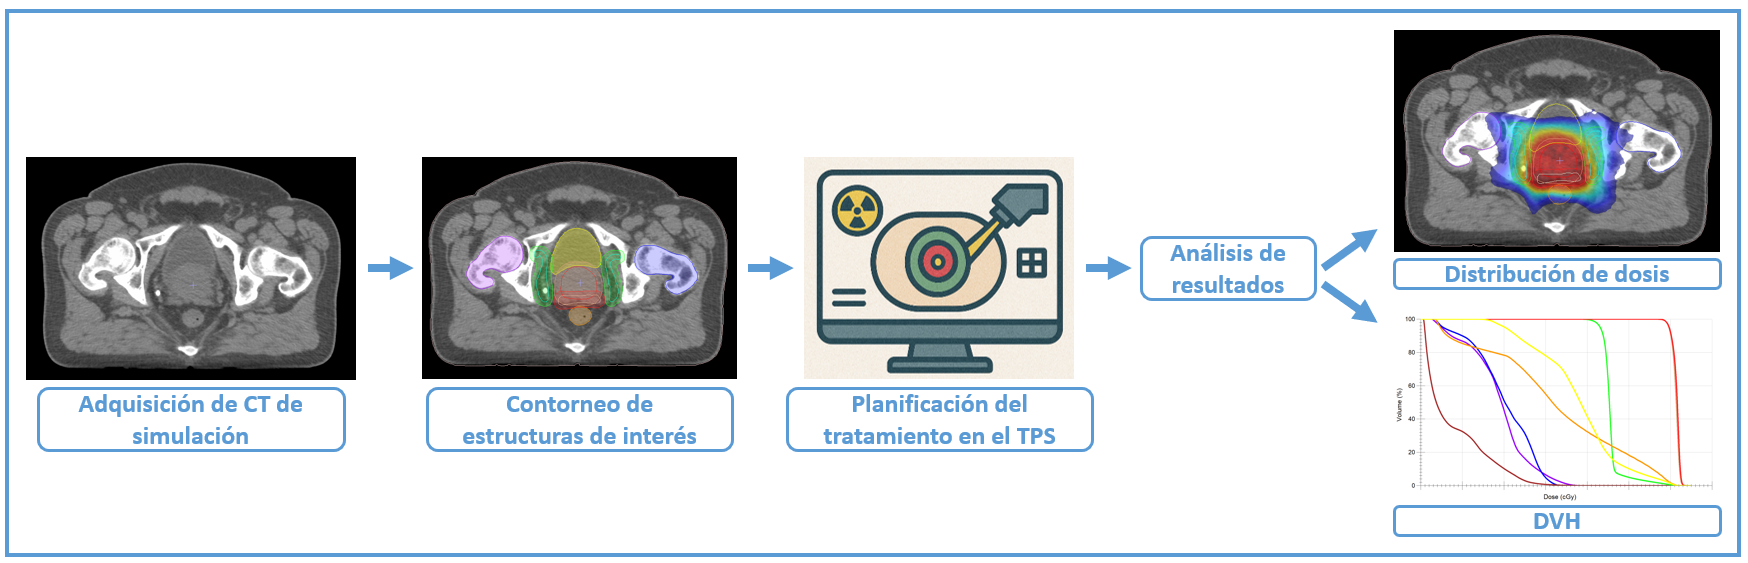
\includegraphics[width=1\textwidth]{./Figuras/Fig1-FlujoDeTrabajo.png}
\caption{Flujo de trabajo de la planificación de un tratamiento de radioterapia.}
\label{fig:FlujoTrabajo}
\end{figure}

\vspace{15px}

Estas imágenes de tomografía se cargan en el TPS, donde el médico radioterapeuta dibuja las estructuras de interés: órganos de riesgo (OAR, del inglés \textit{Organs At Risk}) y volúmenes blanco a tratar. Además, el médico prescribe la dosis terapéutica y las dosis límite de los OARs. 

A partir de esta información, que es específica para cada paciente, el físico médico realiza la planificación del tratamiento. Ésta consiste en determinar los diversos parámetros del equipo, tales como energía, ángulos de incidencia, colimación, rotación del equipo e intensidad, con el objetivo de dispensar la dosis en el volumen blanco prescripta por el médico, minimizando la dosis en los tejidos sanos y cumpliendo con las restricciones indicadas para cada OAR.

Usualmente, los tratamientos de próstata de alto riesgo (próstata + vesículas seminales + ganglios linfáticos) se realizan con la técnica VMAT (Terapia en Arco Modulada Volumétricamente), en la que el equipo gira en forma continua alrededor del paciente mientras dispensa el tratamiento. Para esta técnica se utiliza planificación inversa, que consiste en indicarle al planificador, mediante diversas funciones de costo, los objetivos dosimétricos en cuanto a cobertura del volumen blanco y restricciones de dosis de los OAR. A partir de éstas, el TPS ajusta los parámetros del equipo para lograr estos objetivos.

La planificación de un tratamiento VMAT de próstata de alto riesgo es un proceso iterativo, que demanda una gran cantidad de tiempo y de recursos. En cada iteración, se analizan los resultados obtenidos y, en función de lo observado, se ajustan los diversos parámetros y las funciones de costo configuradas en el TPS. 

El análisis del plan radica en la revisión de la distribución de dosis sobre el paciente (mediante curvas de isodosis) y en el análisis del DVH. Este último consiste en un histograma acumulado de la dosis en función del volumen para cada OAR (ej. recto y vejiga) y para los volúmenes a tratar (ej. próstata). Mediante su análisis, es posible verificar si las restricciones indicadas por el médico se cumplen (ej. dosis máxima, dosis media, un porcentaje de volumen con cierta dosis como máximo, etc). 

Los resultados que se obtienen están asociados a los parámetros configurados para el tratamiento, pero dependerán en gran medida de la anatomía propia del paciente. Por ejemplo, para una configuración similar del tratamiento, si un paciente tiene la vejiga vacía recibirá más dosis que un paciente con la vejiga llena, ya que en el primer caso habrá más volumen de vejiga cercano a la zona a tratar.

El objetivo de este trabajo consiste en lograr predecir el DVH que se obtendrá a partir de la imagen de tomografía del paciente y el contorneo de estructuras de interés. La predicción del DVH previa a la planificación de un tratamiento permitirá conocer de antemano los resultados posibles de obtener para ese paciente en base a su anatomía específica. Con esta información previa, se busca disminuir la cantidad de iteraciones que requiere el proceso, de manera de optimizar el tiempo y recursos invertidos en cada planificación de tratamiento. 

En la figura \ref{fig:DiagBloques} se observa el flujo de trabajo propuesto para cumplir con este objetivo. Se utilizarán redes neuronales convolucionales (CNN, del inglés \textit{Convolutional Neural Network}) preentrenadas, que tomen como entrada las imágenes de CT junto con los contornos de pacientes históricos, y como salida el DVH asociado al plan de tratamiento de ese caso. 

\vspace{10px}

\begin{figure}[!htpb]
\centering 
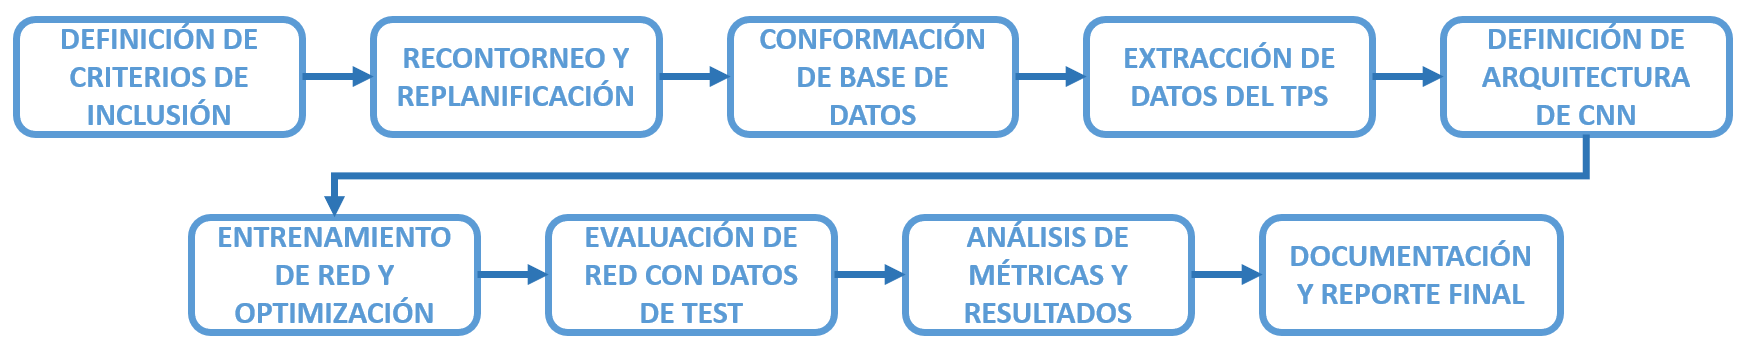
\includegraphics[width=1\textwidth]{./Figuras/Fig2-DiagramaBloques.png}
\caption{Flujo de trabajo propuesto para la predicción de DVH utilizando CNN.}
\label{fig:DiagBloques}
\end{figure}

\vspace{15px}

En una primera etapa, será necesario realizar un análisis exhaustivo de la base de datos actual. Dado que los protocolos de tratamiento se actualizan de manera continua, se deberán estudiar y definir los criterios de selección para determinar los pacientes a incluir en este trabajo. En caso de que el volumen de datos no sea suficiente, se considerará la inclusión de pacientes tratados bajo protocolos previos, recontorneándolos y replanificándolos con el protocolo actual, de modo de homogenizar la base de datos y garantizar su utilidad para el entrenamiento.

Una vez conformada la base de datos específica para este trabajo, se extraerán los datos del TPS y se procederá al entrenamiento del modelo basado en CNN. Se realizará un análisis bibliográfico para identificar la arquitectura más adecuada para la red, y se valorará el uso de técnicas de \textit{transfer learning} que permitan aprovechar modelos preentrenados. El desempeño del modelo se validará frente a nuevos datos mediante métricas cuantitativas que permitan evaluar objetivamente su capacidad predictiva. Finalmente, se documentará todo el trabajo realizado y se reportarán los resultados obtenidos.

\section{2. Identificación y análisis de los interesados}
\label{sec:interesados}

\begin{table}[ht]
%\caption{Identificación de los interesados}
%\label{tab:interesados}
\begin{tabularx}{\linewidth}{@{}|l|>{\hsize=1\hsize}X|>{\hsize=0.6\hsize}X|>{\hsize=1.4\hsize}X|@{}}
\hline
\rowcolor[HTML]{C0C0C0} 
Rol           & Nombre y Apellido  & Organización 	& Puesto 	\\ \hline
Cliente       & \clientename       &\empclientename	& Responsable médica de Servicio de Radioterapia       	\\ \hline
Impulsor      & Mg. Lara Negrin   &\empclientename 	& Responsable de Departamento de Investigación Traslacional       	\\ \hline
Responsable   & \authorname        &\empclientename 	& Alumna 	\\ \hline
Colaboradores & -                  &\empclientename 	& Equipo de médicas radioterapeutas, físicos médicos y técnicos dosimetristas del Servicio de Radioterapia       	\\ \hline
Orientador 1  & \supname	       &\empclientename 	& Director del Trabajo Final \\ \hline
Orientador 2  & Mg. Roy Lápera   &\empclientename 	& Codirector del Trabajo Final \\ \hline
Usuario final & Lic. Fernando Lisa &\empclientename	& Responsable físico de Servicio de Radioterapia       	\\ \hline
\end{tabularx}
\end{table}

\begin{itemize}
	\item Cliente: es la responsable médica del servicio. Valora la optimización del tiempo que transcurre entre la admisión del paciente y el inicio del tratamiento, sin afectar la calidad.
	\item Impulsor: responsable del Departamento de Investigación Traslacional. Valora la investigación, el desarrollo y las actividades académicas en la institución. Además, puede asistir en la presentación del trabajo al Comité de Docencia e Investigación (CDI) de la institución, y al Comité de Evaluación Ética de Proyectos de Investigación en Salud Humana (CEEPISH) de la provincia de Río Negro. 
	\item Colaboradores: el equipo de médicas radioterapeutas, físicos médicos y técnicos dosimetristas del servicio de Radioterapia, que asistirán en el recontorneo y replanificación de los pacientes que se requieran para incluir en la base de datos.
	\item Orientador 1: forma parte del Departamento de Investigación Traslacional, y trabaja en la aplicación de tecnologías computacionales avanzadas en salud. Se especializa en el ámbito del procesamiento de imágenes médicas y física médica computacional, y tiene amplia experiencia en docencia y en dirección de trabajos finales de carrera.
	\item Orientador 2: tiene amplia experiencia como físico médico en el servicio de Radioterapia. Además, tiene formación en el ámbito de la ciencia de datos y la inteligencia artificial, por lo que puede aportar tanto en esas áreas como desde el conocimiento del dominio.
	\item Usuario final: es el responsable físico del servicio de Radioterapia. Es quien podrá determinar la utilidad y la aplicabilidad de este proyecto en el flujo clínico. Deben incluirse también como usuarios finales el resto del equipo de físicos médicos especialistas en radioterapia y técnicos dosimetristas.
\end{itemize}


\section{3. Propósito del proyecto}
\label{sec:proposito}

Este proyecto tiene como objetivo predecir el DVH de los OAR de una planificación de un tratamiento de radioterapia de próstata, a partir de las imágenes de la tomografía de simulación de un paciente y del contorneo de estructuras de interés. Contar con esta predicción previa a comenzar la planificación permitirá optimizar el tiempo y recursos invertidos en esta etapa. Esto contribuirá a reducir el tiempo que transcurre entre la CT de planificación y el inicio del tratamiento, lo cual es especialmente crítico en el contexto clínico.

\section{4. Alcance del proyecto}
\label{sec:alcance}

El alcance del proyecto incluye:
\begin{itemize}
	\item Ingeniería de datos: análisis exhaustivo de la base de datos actual, definición de criterios de inclusión y exclusión, recontorneo de estructuras y replanificación de tratamientos en casos específicos, anonimización de los datos, conformación de la base de datos específica del proyecto, extracción y procesamiento de datos del TPS.
	\item Revisión bibliográfica: estudio del estado del arte en predicción de DVH, arquitecturas de redes convolucionales y técnicas de transfer learning aplicadas al ámbito de la radioterapia.
	\item Implementación de modelos: propuesta de la arquitectura de la CNN, entrenamiento y optimización del modelo, ajuste de hiperparámetros, exploración del impacto de distintas configuraciones de entrada (CT, contornos, combinaciones).
	\item Evaluación del desempeño: validación del modelo con nuevo conjunto de casos, análisis de métricas cuantitativas de desempeño, comparación con resultados reportados en la bibliografía.
	\item Documentación y reporte: registro detallado del proceso, justificación de decisiones técnicas y presentación de resultados intermedios y finales.
	
\end{itemize}

A su vez, el alcance no incluye:
\begin{itemize}
	\item Integración ni implementación del modelo en el flujo clínico actual.
	\item Validación prospectiva en pacientes en curso de tratamiento.
	
\end{itemize}


\section{5. Supuestos del proyecto}
\label{sec:supuestos}

Para el desarrollo del presente proyecto se asume:

\begin{itemize}
	\item Disponibilidad de tiempo: se contará con el tiempo suficiente para llevar adelante las distintas etapas del proyecto dentro del ámbito laboral, considerando las limitaciones propias de la práctica clínica y la necesidad de compatibilizar las actividades asistenciales con las de investigación.
	\item Recursos humanos: se dispondrá del equipo interdisciplinario necesario (médicos radioterapeutas, físicos médicos y técnicos dosimetristas) para realizar el recontorneo y/o la replanificación de los casos requeridos en la construcción de la base de datos.
	\item Recursos materiales y tecnológicos: se dispondrá de los recursos computacionales adecuados, incluyendo acceso a hardware especializado (por ejemplo, GPU de alto rendimiento) para el entrenamiento y la validación de los modelos de redes neuronales.
	\item Apoyo institucional: se contará con el respaldo de la institución en lo relativo al acceso a datos clínicos anonimizados, la utilización de infraestructura y la promoción del desarrollo de herramientas basadas en inteligencia artificial en el ámbito de la radioterapia.
	\item Disponibilidad y calidad de los datos: los datos extraídos del TPS y de los sistemas de registro se encontrarán completos, consistentes y con la calidad suficiente para permitir su utilización en el entrenamiento del modelo.
	\item Cumplimiento normativo y ético: el proyecto se desarrollará en conformidad con las normativas vigentes en materia de ética en investigación clínica y protección de datos personales, garantizando la anonimización y el resguardo de la información de los pacientes.
\end{itemize}


\section{6. Requerimientos}
\label{sec:requerimientos}

\begin{enumerate}
	\item Requerimientos funcionales:
		\begin{enumerate}
			\item El sistema deberá recibir la CT del paciente y las estructuras de interés y debe devolver el DVH predicho.
			\item El modelo deberá ser accesible desde la estación de trabajo del TPS.
			\item La predicción deberá realizarse en un tiempo corto (del orden de minutos).
		\end{enumerate}
	\item Requerimientos de datos:
		\begin{enumerate}
			\item El sistema será entrenado con tratamientos de pacientes realizados en la institución.
			\item Se trabajará con datos anonimizados y se garantizará el resguardo de la información de los pacientes.
			\item Se deberá contar con la información completa para el entrenamiento, que comprende: CT de planificación, contorneo de estructuras de interés y DVH.
		\end{enumerate}
	\item Requerimientos no funcionales:
		\begin{enumerate}
			\item Los pacientes incluidos en este proyecto deben haber dado su consentimiento para el uso de sus datos para fines académicos y de investigación.
			\item El uso de imágenes, planificaciones, y datos de pacientes retrospectivos para este proyecto deberá ser evaluado y aprobado por el Comité de Evaluación Ética de Proyectos de Investigación en Salud Humana (CEEPISH) de la provincia de Río Negro.
			\item El proyecto deberá ser evaluado y aprobado por el Comité de Docencia e Investigación (CDI) de la institución.
		\end{enumerate}
	\item Requerimientos de documentación:
		\begin{enumerate}
			\item Se elaborará un informe detallado del trabajo realizado, incluyendo el procesamiento de los datos, la arquitectura de la red, el proceso de entrenamiento y el análisis de los resultados.
			\item Se confeccionará un instructivo para el uso de la red entrenada y la interpretación de la predicción.
		\end{enumerate}
	\item Requerimientos de \textit{testing}:
		\begin{enumerate}
			\item Se compararán los resultados de la predicción con los resultados de casos que no hayan sido utilizados en el entrenamiento.
			\item Se contrastarán los resultados obtenidos con los reportados en la bibliografía.
			\item Se valorará el tiempo requerido para la planificación con y sin la implementación del modelo en conjunto con el usuario.
		\end{enumerate}
	
\end{enumerate}

\section{7. Historias de usuarios (\textit{Product backlog})}
\label{sec:backlog}

A continuación, se analizarán tres historias de usuario, que describen en forma simple qué necesitan distintos interesados desde su rol y con qué objetivo. Cada una de estas historias se evaluará según tres dimensiones: dificultad (cantidad de trabajo estimado), complejidad (nivel técnico) e incertidumbre (riesgo o novedad). El puntaje se asignará según el siguiente criterio:

\vspace{10px}

\begin{table}[ht]
\centering
\setlength{\tabcolsep}{3pt}
\begin{tabularx}{0.85\linewidth}{@{}|>{\centering\arraybackslash}X|>{\centering\arraybackslash}X|>{\centering\arraybackslash}X|>{\centering\arraybackslash}X|@{}}
\hline
\rowcolor[HTML]{C0C0C0}
Criterio      & Baja & Media & Alta \\ \hline
Dificultad    & 1    & 3     & 5    \\ \hline
Complejidad   & 1    & 5     & 8    \\ \hline
Incertidumbre & 1    & 3     & 5    \\ \hline
\end{tabularx}
\end{table}


\vspace{10px}

Finalmente, para obtener el total de \textit{story points} se sumarán los valores de las tres dimensiones, y se redondeará el total al número superior más próximo de la serie de Fibonacci.

\begin{itemize}
\item Historia 1: Como responsable del servicio de radioterapia, busco optimizar el tiempo invertido en todas las etapas del proceso, para minimizar el tiempo transcurrido entre la admisión del paciente y el inicio de su tratamiento.

\textit{Story points}: 21 (dificultad: 5, complejidad: 8, incertidumbre: 5, total: 18)

\item Historia 2: Como médico radioterapeuta, me gustaría saber si la prescripción de dosis indicada es viable, para decidir si debe repetirse la tomografía de planificación modificando la preparación del paciente.

\textit{Story points}: 13 (dificultad: 3, complejidad: 5, incertidumbre: 3, total: 11)

\item Historia 3: Como físico médico, quiero conocer el resultado posible de un plan para determinar los mejores parámetros a utilizar en la planificación del tratamiento y reducir la cantidad de iteraciones necesarias.

\textit{Story points}: 21 (dificultad: 5, complejidad: 8, incertidumbre: 3, total: 16)
\end{itemize}


\section{8. Entregables principales del proyecto}
\label{sec:entregables}

Los entregables del proyecto son :

\begin{itemize}
	\item Documento de planificación del proyecto.
	\item Base de datos anonimizada y procesada.
	\item Repositorio del código desarrollado.
	\item Instructivo de uso de la red entrenada.
	\item Memoria del trabajo final.
	\item Presentación final
\end{itemize}

\section{9. Desglose del trabajo en tareas}
\label{sec:wbs}

\begin{enumerate}
\item Análisis bibliográfico (40 h)
	\begin{enumerate}
	\item Búsqueda y análisis de bibliografía sobre predicción de DVH (20 h)
	\item Búsqueda y análisis de bibliografía sobre arquitecturas de CNN y \textit{transfer learning} (20 h)
	\end{enumerate}
\item Cumplimiento de requerimientos normativos y éticos (25 h)
	\begin{enumerate}
	\item Presentación del proyecto a CDI institucional (10 h)
	\item Confección de documentación para presentación a CEEPISH (10 h)
	\item Recopilación de consentimientos informados de posibles pacientes a incluir (5 h)
	\end{enumerate}
\item Conformación de base de datos (200 h)
	\begin{enumerate}
	\item Definición de criterios de inclusión en el proyecto (2 h)
	\item Confección de listado de pacientes posibles (3 h)
	\item Análisis de cumplimiento de criterios en listado de pacientes posibles (10 h)
	\item Armado de nueva base de datos específica para el proyecto (10 h)
	\item Recontorneo y replanificación de pacientes para incluir en base de datos (160 h)
	\item Anonimización de base de datos (15 h)
	\end{enumerate}
\item Evaluación de requerimientos de hardware (5 h)
	\begin{enumerate}
	\item Análisis de necesidad de cluster externo en función de tamaño de la base de datos (5 h)
	\end{enumerate}
\item Extracción de datos del TPS (50 h)
	\begin{enumerate}
	\item Estudio de formato de datos DICOM (10 h)
	\item Desarrollo de código para la extracción de datos necesarios (CT, estructuras, DVH) (40 h)
	\end{enumerate}
\item Desarrollo de CNN (150 h)
	\begin{enumerate}
	\item Definición de arquitectura de CNN (10 h)
	\item Desarrollo de código para entrenamiento y validación de CNN (40 h)
	\item Entrenamiento de CNN y optimización de hiperparámetros (100 h)
	\end{enumerate}
\item Validación (60 h)
	\begin{enumerate}
	\item Evaluación de red con datos de test (20 h)
	\item Análisis de métricas y resultados obtenidos (30 h)
	\item Comparación con resultados reportados en la bibliografía (10 h)
	\end{enumerate}
\item Documentación final (80 h)
	\begin{enumerate}
	\item Elaboración de instructivo de uso (10 h)
	\item Revisión de repositorio de código desarrollado y documentación del código (10 h)
	\item Elaboración de informes de avance (10 h)
	\item Elaboración de memoria de trabajo final (40 h)
	\item Confección de presentación final (10 h)
	\end{enumerate}
\end{enumerate}

Cantidad total de horas: 610 h.

\section{10. Diagrama de Activity On Node}
\label{sec:AoN}

\begin{consigna}{red}
Armar el AoN a partir del WBS definido en la etapa anterior.

Una herramienta simple para desarrollar los diagramas es el Draw.io (\url{https://app.diagrams.net/}).
\href{https://app.diagrams.net}{Draw.io}


\begin{figure}[htpb]
\centering 
\includegraphics[width=.8\textwidth]{./Figuras/AoN.png}
\caption{Diagrama de \textit{Activity on Node}.}
\label{fig:AoN}
\end{figure}

Indicar claramente en qué unidades están expresados los tiempos.
De ser necesario indicar los caminos semi críticos y analizar sus tiempos mediante un cuadro.
Es recomendable usar colores y un cuadro indicativo describiendo qué representa cada color.

\end{consigna}

\section{11. Diagrama de Gantt}
\label{sec:gantt}

\begin{consigna}{red}
Existen muchos programas y recursos \textit{online} para hacer diagramas de Gantt, entre los cuales destacamos:

\begin{itemize}
\item Planner
\item GanttProject
\item Trello + \textit{plugins}. En el siguiente link hay un tutorial oficial: \\ \url{https://blog.trello.com/es/diagrama-de-gantt-de-un-proyecto}
\item Creately, herramienta online colaborativa. \\\url{https://creately.com/diagram/example/ieb3p3ml/LaTeX}
\item Se puede hacer en latex con el paquete \textit{pgfgantt}\\ \url{http://ctan.dcc.uchile.cl/graphics/pgf/contrib/pgfgantt/pgfgantt.pdf}
\end{itemize}

Pegar acá una captura de pantalla del diagrama de Gantt, cuidando que la letra sea suficientemente grande como para ser legible. 
Si el diagrama queda demasiado ancho, se puede pegar primero la ``tabla'' del Gantt y luego pegar la parte del diagrama de barras del diagrama de Gantt.

Configurar el software para que en la parte de la tabla muestre los códigos del EDT (WBS).\\
Configurar el software para que al lado de cada barra muestre el nombre de cada tarea.\\
Revisar que la fecha de finalización coincida con lo indicado en el Acta Constitutiva.

En la figura \ref{fig:gantt}, se muestra un ejemplo de diagrama de gantt realizado con el paquete de \textit{pgfgantt}. 
En la plantilla pueden ver el código que lo genera y usarlo de base para construir el propio.

Las fechas pueden ser calculadas utilizando alguna de las herramientas antes citadas. Sin embargo, el siguiente ejemplo
fue elaborado utilizando 
\href{https://docs.google.com/spreadsheets/d/1fBz8NhSpc4tkkhz3KjJCbh1nR_ltDkfEcZi4tZXduqs}{esta hoja de cálculo}.

Es importante destacar que el ancho del diagrama estará dado por la longitud del texto utilizado para las tareas 
(Ejemplo: tarea 1, tarea 2, etcétera) y el valor \textit{x unit}. Para mejorar la apariencia del diagrama, es necesario
ajustar este valor y, quizás, acortar los nombres de las tareas.

\begin{figure}[htpb]
  \begin{center}
    \begin{ganttchart}[
      time slot unit=day,
      time slot format=isodate,
      x unit=0.038cm,
      y unit title=0.7cm,
      y unit chart=0.6cm,
      milestone/.append style={xscale=4}
      ]{2021-03-05}{2021-12-16}
      \gantttitlecalendar*{2021-03-05}{2021-12-16}{year} \\
      \gantttitlecalendar*{2021-03-05}{2021-12-16}{month} \\
      \ganttgroup{Duración Total}{2021-03-05}{2021-12-16} \\
      %%%%%%%%%%%%%%%%%Organización
      \ganttgroup{Organización}{2021-03-05}{2021-04-16} \\
      \ganttbar{Planificación del proyecto}{2021-03-05}{2021-04-15} \\
      %%%%%%%%%%%%%%%%%Ejecución
      \ganttgroup{Ejecución}{2021-04-16}{2021-10-21} \\
      \ganttbar{Tarea 1}{2021-04-16}{2021-04-29} \\
      \ganttbar{Tarea 2}{2021-04-30}{2021-05-13} \\
      \ganttbar{Tarea 3}{2021-05-14}{2021-05-27} \\
      \ganttbar{Tarea 4}{2021-05-28}{2021-07-12} \\
      \ganttbar{Tarea 5}{2021-07-13}{2021-08-09} \\
      \ganttbar{Tarea 6}{2021-08-10}{2021-09-23} \\
      \ganttbar{Tarea 7}{2021-09-24}{2021-09-30} \\
      \ganttbar{Tarea 8}{2021-10-01}{2021-10-14} \\
      \ganttbar{Tarea 9}{2021-10-15}{2021-10-21} \\
      % %%%%%%%%%%%%%%%%%Finalización
      \ganttgroup{Finalización}{2021-10-22}{2021-12-16} \\
      \ganttbar{Memoria v1}{2021-10-22}{2021-11-04} \\
      \ganttbar{Memoria v2}{2021-11-05}{2021-11-18} \\
      \ganttbar{Memoria final}{2021-11-19}{2021-12-02} \\
      % La fecha del siguiente milestone es la fecha en que terminamos la memoria
      \ganttmilestone{Enviar memoria al director}{2021-12-02} \\
      \ganttbar{Elaborar la presentación}{2021-12-03}{2021-12-16} \\
      \ganttmilestone{Ensayo de la presentación}{2021-12-16} \\
      %%%%%%%%%%%%%%%%%%%%%%%%%%%%%%%%%%%%%%%%%%%%%%%%%%%%%%%%%%%%%%%
    \end{ganttchart}
  \end{center}
  \caption{Diagrama de gantt de ejemplo}
  \label{fig:gantt}
\end{figure}


\begin{landscape}
\begin{figure}[htpb]
\centering 
\includegraphics[height=.85\textheight]{./Figuras/Gantt-2.png}
\caption{Ejemplo de diagrama de Gantt (apaisado).} %Modificar este título acorde.
\label{fig:diagGantt}
\end{figure}

\end{landscape}

\end{consigna}


\section{12. Presupuesto detallado del proyecto}
\label{sec:presupuesto}

\begin{consigna}{red}
Si el proyecto es complejo entonces separarlo en partes:
\begin{itemize}
	\item Un total global, indicando el subtotal acumulado por cada una de las áreas.
	\item El desglose detallado del subtotal de cada una de las áreas.
\end{itemize}

IMPORTANTE: No olvidarse de considerar los COSTOS INDIRECTOS.

Incluir la aclaración de si se emplea como moneda el peso argentino (ARS) o si se usa moneda extranjera (USD, EUR, etc). Si es en moneda extranjera se debe indicar la tasa de conversión respecto a la moneda local en una fecha dada.

\end{consigna}

\begin{table}[htpb]
\centering
\begin{tabularx}{\linewidth}{@{}|X|c|r|r|@{}}
\hline
\rowcolor[HTML]{C0C0C0} 
\multicolumn{4}{|c|}{\cellcolor[HTML]{C0C0C0}COSTOS DIRECTOS} \\ \hline
\rowcolor[HTML]{C0C0C0} 
Descripción &
  \multicolumn{1}{c|}{\cellcolor[HTML]{C0C0C0}Cantidad} &
  \multicolumn{1}{c|}{\cellcolor[HTML]{C0C0C0}Valor unitario} &
  \multicolumn{1}{c|}{\cellcolor[HTML]{C0C0C0}Valor total} \\ \hline
 &
  \multicolumn{1}{c|}{} &
  \multicolumn{1}{c|}{} &
  \multicolumn{1}{c|}{} \\ \hline
 &
  \multicolumn{1}{c|}{} &
  \multicolumn{1}{c|}{} &
  \multicolumn{1}{c|}{} \\ \hline
\multicolumn{1}{|l|}{} &
   &
   &
   \\ \hline
\multicolumn{1}{|l|}{} &
   &
   &
   \\ \hline
\multicolumn{3}{|c|}{SUBTOTAL} &
  \multicolumn{1}{c|}{} \\ \hline
\rowcolor[HTML]{C0C0C0} 
\multicolumn{4}{|c|}{\cellcolor[HTML]{C0C0C0}COSTOS INDIRECTOS} \\ \hline
\rowcolor[HTML]{C0C0C0} 
Descripción &
  \multicolumn{1}{c|}{\cellcolor[HTML]{C0C0C0}Cantidad} &
  \multicolumn{1}{c|}{\cellcolor[HTML]{C0C0C0}Valor unitario} &
  \multicolumn{1}{c|}{\cellcolor[HTML]{C0C0C0}Valor total} \\ \hline
\multicolumn{1}{|l|}{} &
   &
   &
   \\ \hline
\multicolumn{1}{|l|}{} &
   &
   &
   \\ \hline
\multicolumn{1}{|l|}{} &
   &
   &
   \\ \hline
\multicolumn{3}{|c|}{SUBTOTAL} &
  \multicolumn{1}{c|}{} \\ \hline
\rowcolor[HTML]{C0C0C0}
\multicolumn{3}{|c|}{TOTAL} &
   \\ \hline
\end{tabularx}%
\end{table}


\section{13. Gestión de riesgos}
\label{sec:riesgos}

\begin{consigna}{red}
a) Identificación de los riesgos (al menos cinco) y estimación de sus consecuencias:
 
Riesgo 1: detallar el riesgo (riesgo es algo que si ocurre altera los planes previstos de forma negativa)
\begin{itemize}
	\item Severidad (S): mientras más severo, más alto es el número (usar números del 1 al 10).\\
	Justificar el motivo por el cual se asigna determinado número de severidad (S).
	\item Probabilidad de ocurrencia (O): mientras más probable, más alto es el número (usar del 1 al 10).\\
	Justificar el motivo por el cual se asigna determinado número de (O). 
\end{itemize}   

Riesgo 2:
\begin{itemize}
	\item Severidad (S): X.\\
	Justificación...
	\item Ocurrencia (O): Y.\\
	Justificación...
\end{itemize}

Riesgo 3:
\begin{itemize}
	\item Severidad (S):  X.\\
	Justificación...
	\item Ocurrencia (O): Y.\\
	Justificación...
\end{itemize}


b) Tabla de gestión de riesgos:      (El RPN se calcula como RPN=SxO)

\begin{table}[htpb]
\centering
\begin{tabularx}{\linewidth}{@{}|X|c|c|c|c|c|c|@{}}
\hline
\rowcolor[HTML]{C0C0C0} 
Riesgo & S & O & RPN & S* & O* & RPN* \\ \hline
       &   &   &     &    &    &      \\ \hline
       &   &   &     &    &    &      \\ \hline
       &   &   &     &    &    &      \\ \hline
       &   &   &     &    &    &      \\ \hline
       &   &   &     &    &    &      \\ \hline
\end{tabularx}%
\end{table}

Criterio adoptado: 

Se tomarán medidas de mitigación en los riesgos cuyos números de RPN sean mayores a...

Nota: los valores marcados con (*) en la tabla corresponden luego de haber aplicado la mitigación.

c) Plan de mitigación de los riesgos que originalmente excedían el RPN máximo establecido:
 
Riesgo 1: plan de mitigación (si por el RPN fuera necesario elaborar un plan de mitigación).
  Nueva asignación de S y O, con su respectiva justificación:
  \begin{itemize}
	\item Severidad (S*): mientras más severo, más alto es el número (usar números del 1 al 10).
          Justificar el motivo por el cual se asigna determinado número de severidad (S).
	\item Probabilidad de ocurrencia (O*): mientras más probable, más alto es el número (usar del 1 al 10).
          Justificar el motivo por el cual se asigna determinado número de (O).
	\end{itemize}

Riesgo 2: plan de mitigación (si por el RPN fuera necesario elaborar un plan de mitigación).
 
Riesgo 3: plan de mitigación (si por el RPN fuera necesario elaborar un plan de mitigación).

\end{consigna}


\section{14. Gestión de la calidad}
\label{sec:calidad}

\begin{consigna}{red}
Elija al menos diez requerimientos que a su criterio sean los más importantes/críticos/que aportan más valor y para cada uno de ellos indique las acciones de verificación y validación que permitan asegurar su cumplimiento.

\begin{itemize} 
\item Req \#1: copiar acá el requerimiento con su correspondiente número.

\begin{itemize}
	\item Verificación para confirmar si se cumplió con lo requerido antes de mostrar el sistema al cliente. Detallar.
	\item Validación con el cliente para confirmar que está de acuerdo en que se cumplió con lo requerido. Detallar. 
\end{itemize}

\end{itemize}

Tener en cuenta que en este contexto se pueden mencionar simulaciones, cálculos, revisión de hojas de datos, consulta con expertos, mediciones, etc.  

Las acciones de verificación suelen considerar al entregable como ``caja blanca'', es decir se conoce en profundidad su funcionamiento interno.  

En cambio, las acciones de validación suelen considerar al entregable como ``caja negra'', es decir, que no se conocen los detalles de su funcionamiento interno.

\end{consigna}

\section{15. Procesos de cierre}    
\label{sec:cierre}

\begin{consigna}{red}
Establecer las pautas de trabajo para realizar una reunión final de evaluación del proyecto, tal que contemple las siguientes actividades:

\begin{itemize}
	\item Pautas de trabajo que se seguirán para analizar si se respetó el Plan de Proyecto original:\\
	 - Indicar quién se ocupará de hacer esto y cuál será el procedimiento a aplicar. 
	\item Identificación de las técnicas y procedimientos útiles e inútiles que se emplearon, los problemas que surgieron y cómo se solucionaron:\\
	 - Indicar quién se ocupará de hacer esto y cuál será el procedimiento para dejar registro.
	\item Indicar quién organizará el acto de agradecimiento a todos los interesados, y en especial al equipo de trabajo y colaboradores:\\
	  - Indicar esto y quién financiará los gastos correspondientes.
\end{itemize}

\end{consigna}

\end{document}